
\begin{figure*} [b!]
\begin{tcolorbox}[colframe=black!30!black, colback=white]
\hfill
\begin{subfigure}[r]{0.5\textwidth}
    
\includegraphics[width=\textwidth]{Figures/legend}
  \end{subfigure}
  \vskip\baselineskip
  \hspace{-5mm}
  \begin{subfigure}[b]{0.51\textwidth}
    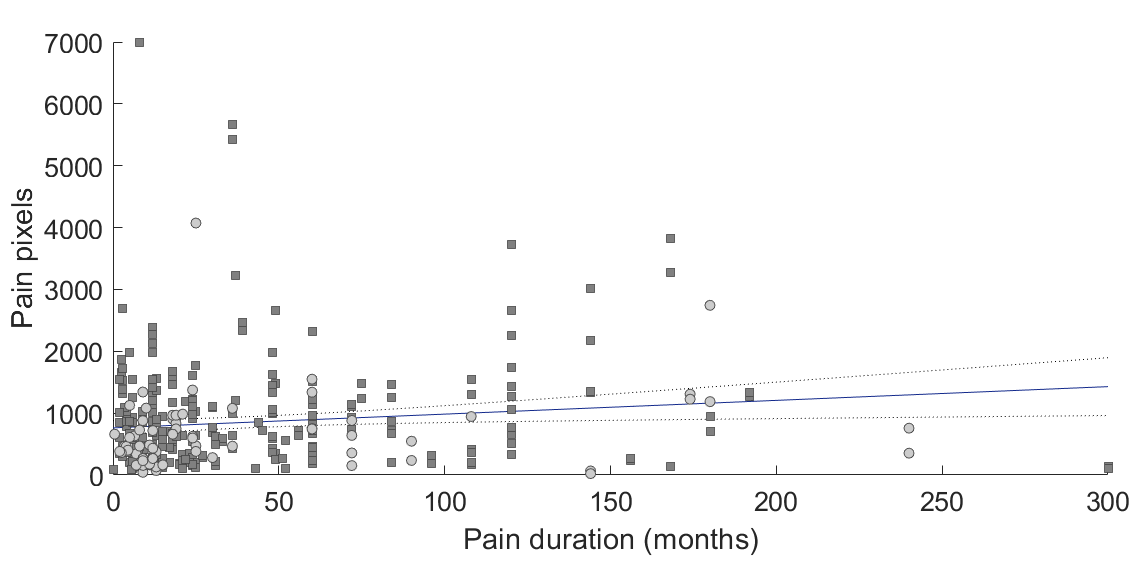
\includegraphics[width=\textwidth]{Figures/durapixel}
    \caption{ }
    \label{fig:1}
  \end{subfigure}
  \hfill
    \hspace{2mm}
  \begin{subfigure}[b]{0.51\textwidth}
    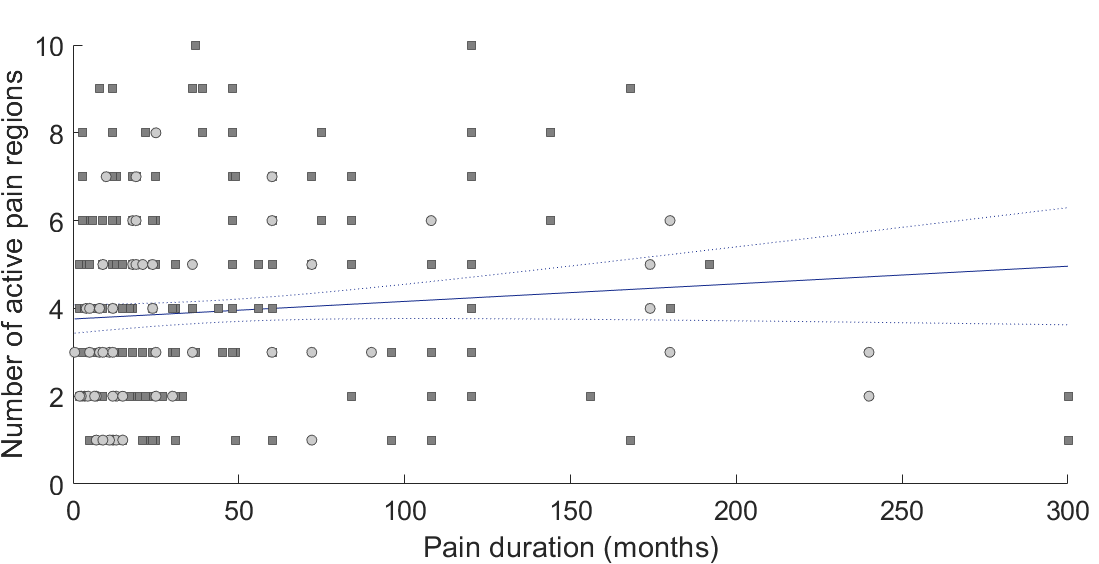
\includegraphics[width=\textwidth]{Figures/duraregion}
       \caption{ }
    \label{fig:2}
  \end{subfigure}
    \vskip\baselineskip
    \hspace{-5mm}
  \begin{subfigure}[b]{0.51\textwidth}
    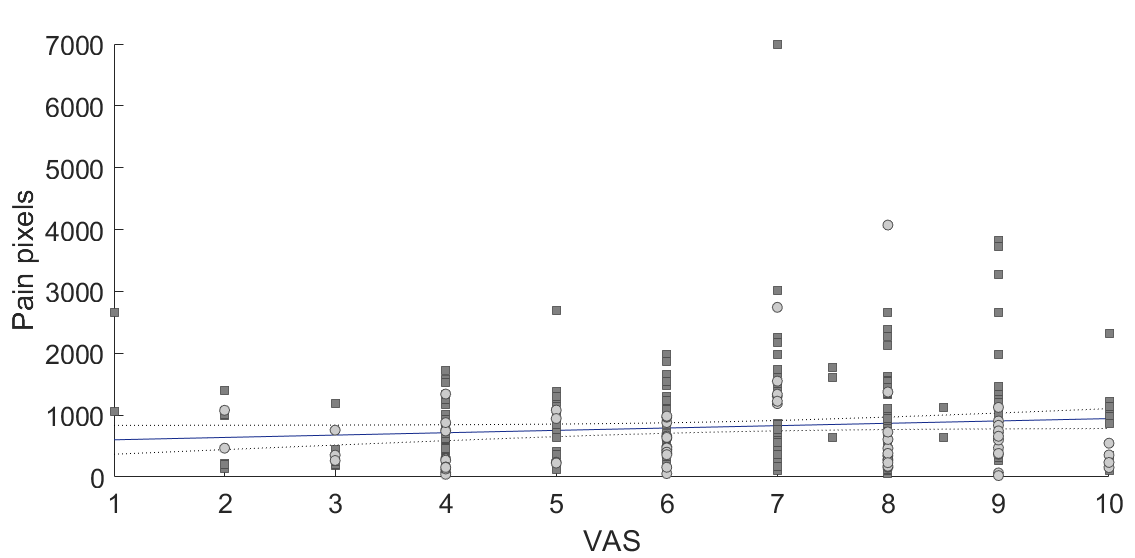
\includegraphics[width=\textwidth]{Figures/vaspixel}
    \caption{}
    \label{fig:3}
  \end{subfigure}
  \hfill
  \hspace{2mm}
  \begin{subfigure}[b]{0.51\textwidth}
    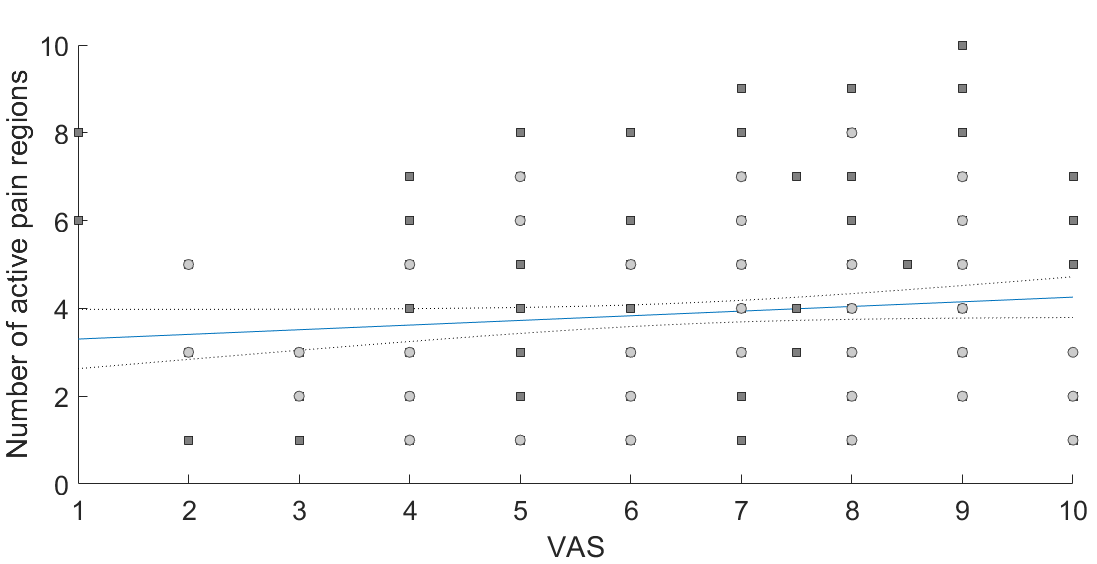
\includegraphics[width=\textwidth]{Figures/vasregion}
       \caption{ }
    \label{fig:4}
  \end{subfigure}  
  \caption{Linear correlations of pain pixels and pain duration (a), active pain regions and pain duration (b), pain pixels and pain intensity indicated in VAS (c), and active pain regions and pain intensity indicated in VAS (d).}
  \label{fig:correlations}
\end{tcolorbox}
\end{figure*}

This section visualizes the results from the linear regressions, and performance of the deep learning models using multiple pain map representations, and different outputs. 
\vspace{-0.3cm}

\subsection{Linear correlations}
The linear regression between simple features, number of pain pixels or active pain regions, and outputs, pain duration or pain intensity, resulted in the plots shown in fig. \ref{fig:correlations}. The $R^2$-values support the nonlinearity, shown in the plots, where correlation fig. \ref{fig:1} resulted in a $R^2 = 0.018$, fig. \ref{fig:2} resulted in $R^2 = 0.008$, fig. \ref{fig:3} resulted in $R^2 = 0.011$ and fig. \ref{fig:4} resulted in $R^2 = 0.011$. 


\begin{table*}[b!]
\centering
\begin{tabular}{@{}llll@{}}
\toprule
\multicolumn{4}{c}{\hspace{2.3cm} Avg. accuracy (\%) \hspace{1cm} Avg. sensitivity (\%) \hspace{1cm} Avg. specificity (\%) \hspace{1cm}                }                                                                                                                                                                         \\ \midrule
\multicolumn{4}{c}{Morphology-representation} \\ \midrule
Pain duration  & \hspace{0.7cm}\begin{tabular}[c]{@{}l@{}}69.44\% \end{tabular} & \hspace{2.6cm} \begin{tabular}[c]{@{}l@{}}56.25\%\end{tabular} & \hspace{2.7cm} \begin{tabular}[c]{@{}l@{}} 80.00\%\end{tabular} \\ %\midrule
Pain intensity & \hspace{0.6cm} \begin{tabular}[c]{@{}l@{}}60.00\% \end{tabular}  & \hspace{2.7cm}\begin{tabular}[c]{@{}l@{}}40.00\% \end{tabular}  & \hspace{2.7cm} \begin{tabular}[c]{@{}l@{}}75.00\%\end{tabular}   \\ \midrule
\multicolumn{4}{c}{Location-representation}                                                                                                                                                                             \\ \midrule
Pain duration  & \hspace{0.6cm} \begin{tabular}[c]{@{}l@{}}35.29\%\end{tabular}  & \hspace{2.6cm} \begin{tabular}[c]{@{}l@{}}0.00\% \end{tabular}  & \hspace{2.7cm} \begin{tabular}[c]{@{}l@{}}100\%\end{tabular}  \\ %\midrule 
Pain intensity & \hspace{0.6cm} \begin{tabular}[c]{@{}l@{}}60.71\% \end{tabular}   & \hspace{2.6cm} \begin{tabular}[c]{@{}l@{}}0.00\% \end{tabular}   & \hspace{2.7cm} \begin{tabular}[c]{@{}l@{}}100\%\end{tabular}  \\ \midrule
\multicolumn{4}{c}{Combined-representation}                                                                                                                                                              \\ \midrule
Pain duration  & \hspace{0.6cm} \begin{tabular}[c]{@{}l@{}}55.56\% \end{tabular}                                                                   & \hspace{2.6cm} \begin{tabular}[c]{@{}l@{}}55.00\%\end{tabular}                                                                & \hspace{2.7cm} \begin{tabular}[c]{@{}l@{}}43.75\%\end{tabular}                                                                                                                                \\% \midrule
Pain intensity & \hspace{0.6cm} \begin{tabular}[c]{@{}l@{}}86.67\% \end{tabular}
&\hspace{2.6cm} \begin{tabular}[c]{@{}l@{}} 75.00\%\end{tabular}                                                               
& \hspace{2.7cm} \begin{tabular}[c]{@{}l@{}} 90.91\%\end{tabular}                                                               
 \\ \bottomrule
\end{tabular}
\caption{Generalization performance of the models, which use the MR, LR, and CR when classifying according to pain duration or pain intensity.}
\label{tab:performance}
\end{table*}


\begin{figure*} [b!]
\begin{tcolorbox}[colframe=black!30!black, colback=white]
    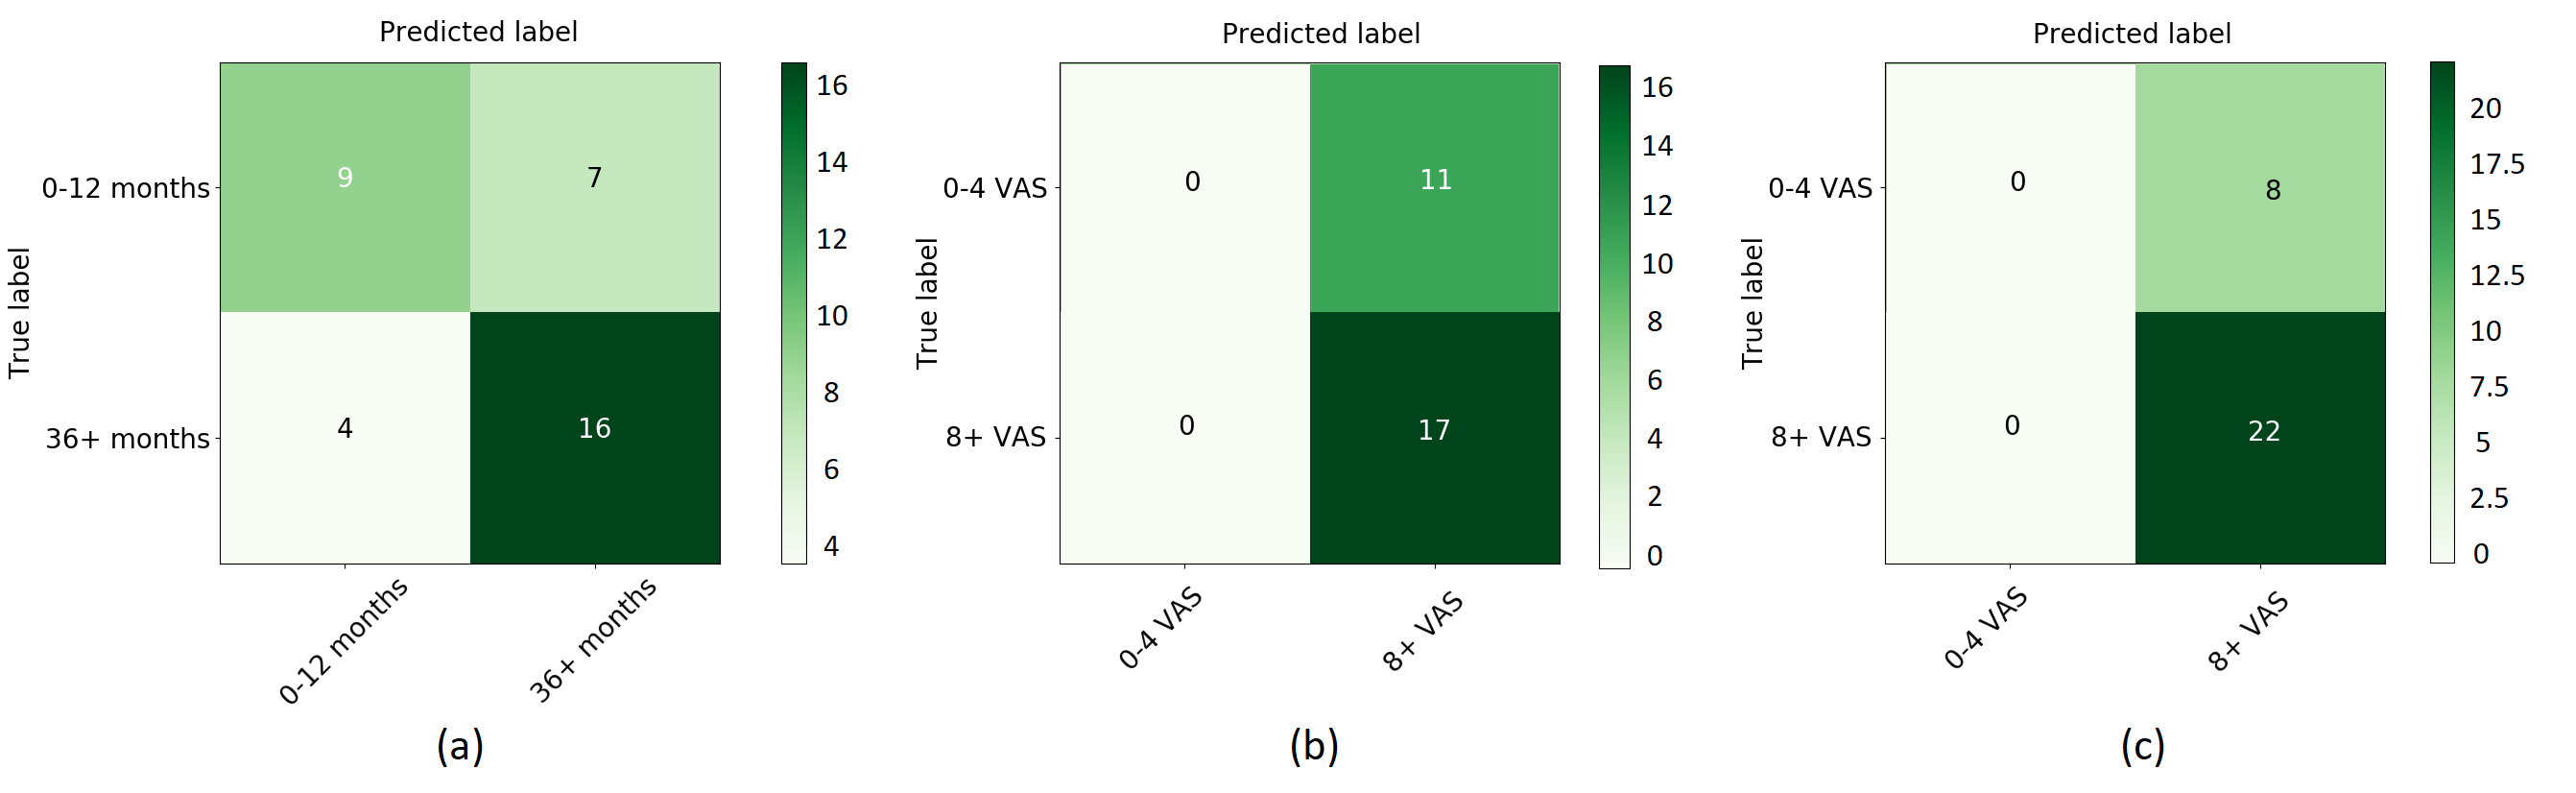
\includegraphics[width=1\textwidth]{Figures/samcon}
  \caption{Confusion matrices of (a) MR classified according to pain duration, (b) classified LR according pain duration, and (c) classified CR according to pain duration.}
  \label{fig:confma}
\end{tcolorbox}
\end{figure*}

\begin{figure*} [t!]
\begin{tcolorbox}[colframe=black!30!black, colback=white]
    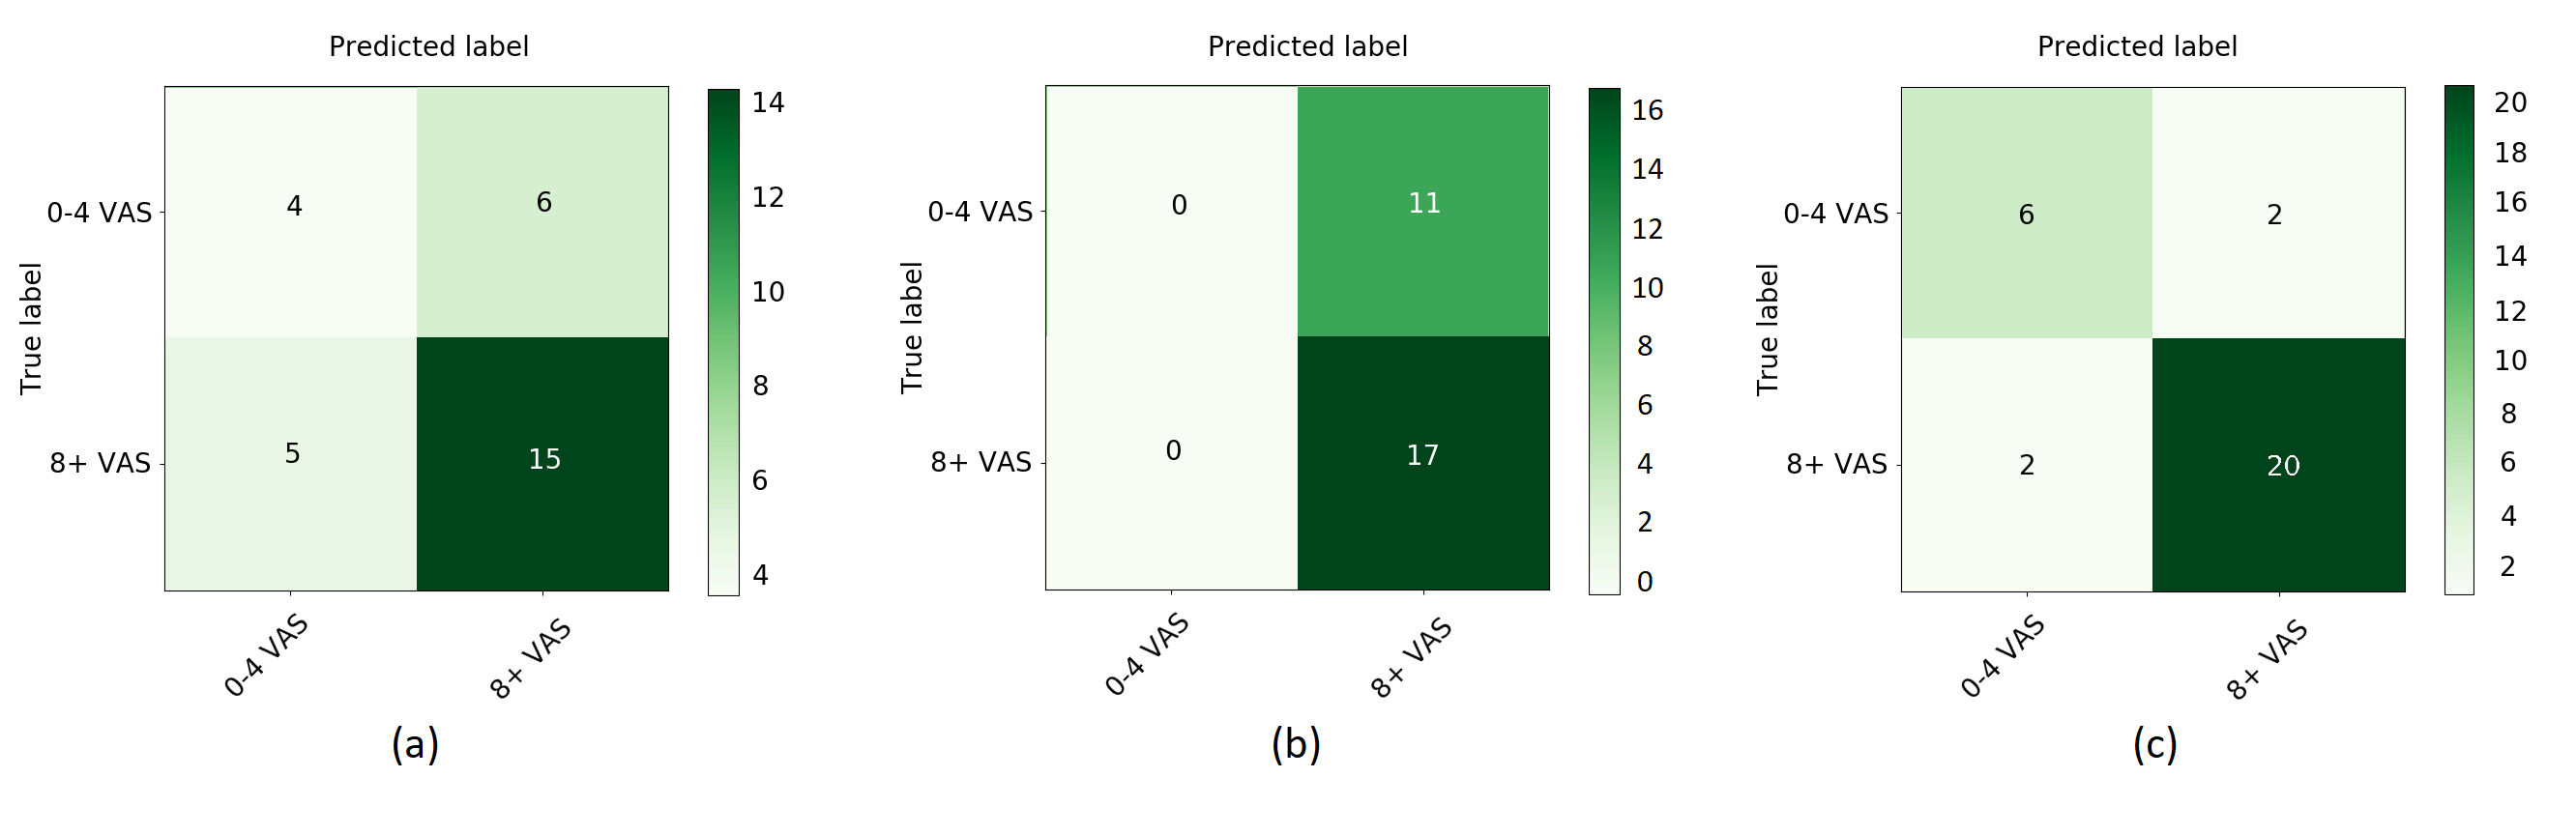
\includegraphics[width=1\textwidth]{Figures/samcon1}
  \caption{Confusion matrices of (a) MR classified according to pain intensity, (b) classified LR according pain intensity, and (c) classified CR according to pain intensity.}
  \label{fig:confma1}
\end{tcolorbox}
\end{figure*}

\subsection{Optimization of the models}
During the optimization, a structured grid search resulted in different hyperparameters according to each model. For the deep learning models including MR and classification type pain duration, the highest performance was obtained with a learning rate of 0.01, the number of nodes of 64, and the epochs and batch size setting of 120 and 20. The models using the MR and pain intensity had the highest performance when using a learning rate of 0.1, 16 nodes, epochs and batch size of 140 and 10. The models including the LR had similar results from the optimization. Learning rate of 0.01, number of nodes at 16, and a number of epochs and batch size of 120 and 20. 
Results of optimization on the models including the CR were almost identical. Both resulted in the best performance with 16 nodes, and with a number of epochs and batch size of 120 and 30, to which the only difference was in the learning rate that for pain duration was 0.1, and 0.001 for pain intensity.

\subsection{Performance of the models}
The average performance accuracy, sensitivity, and specificity of the models during test with new pain maps in different representations are shown in tab. \ref{tab:performance}. \newline
For the pain map representations, confusion matrices were created according to the pain duration as is shown in fig. \ref{fig:confma}, and confusion matrices according to pain intensity as shown in fig. \ref{fig:confma1}.